To perform proper speech recognition, the direction of the sound is important to capture the sound source properly. We localize the sound source by determining the direction of arrival (DOA) with use of the microphone array board with 8 microphones\footnote{\url{https://creator.matrix.one}} of the Matrix Creator.
%depicted in Figure \ref{fig:matrix_one}.
%\begin{figure}[h]
%    \centering
%    %\vspace{-0.3cm}
%	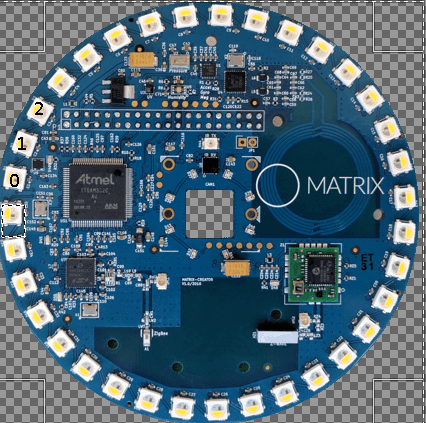
\includegraphics[width = 0.5\linewidth]{Figures/ssl_Matrix_creator.png}
%    %\vspace{-1em}
%	\caption{Matrix One Creator board.}
%	\label{fig:matrix_one}
%    %\vspace{-0.5cm}
%\end{figure}
The detection is done by first calculating the time cross correlation between four pairs of opposing microphones. Second, the microphone pair with the lowest phase shift w.r.t. the opposing microphone is selected as being perpendicular to the source. Finally, the direction of the source can be determined by combining this information with the energy level\footnote{\url{https://github.com/tue-robotics/matrix-creator-hal}} of the microphones. Our software for the DOA detection is available on GitHub, as well as a ROS package\footnote{\url{https://github.com/tue-robotics/matrix_creator_ros}} that exposes the DOA detections via a geometry\_msgs/PoseStamped topic interface. 